% To je predloga za poročila o domačih nalogah pri predmetih, katerih
% nosilec je Blaž Zupan. Seveda lahko tudi dodaš kakšen nov, zanimiv
% in uporaben element, ki ga v tej predlogi (še) ni. Več o LaTeX-u izveš na
% spletu, na primer na http://tobi.oetiker.ch/lshort/lshort.pdf.
%
% To predlogo lahko spremeniš v PDF dokument s pomočjo programa
% pdflatex, ki je del standardne instalacije LaTeX programov.

\documentclass[a4paper,11pt]{article}
\usepackage{a4wide}
\usepackage{fullpage}
\usepackage[utf8x]{inputenc}
\usepackage[slovene]{babel}
\selectlanguage{slovene}
\usepackage[toc,page]{appendix}
\usepackage[pdftex]{graphicx} % za slike
\usepackage{setspace}
\usepackage{color}
\definecolor{light-gray}{gray}{0.95}
\usepackage{listings} % za vključevanje kode
\usepackage{hyperref}
\usepackage{titlesec}
\usepackage{array}
\usepackage{makecell}

\renewcommand{\baselinestretch}{1.2} % za boljšo berljivost večji razmak
\renewcommand{\appendixpagename}{\normalfont\Large\bfseries{Priloge}}


\titleformat{name=\section}[runin]
  {\normalfont\bfseries}{}{0em}{}
\titleformat{name=\subsection}[runin]
  {\normalfont\bfseries}{}{0em}{}


% header
\makeatletter
\def\@maketitle{%
  \noindent
  \begin{minipage}{2in}
  \@author
  \end{minipage}
  \hfill
  \begin{minipage}{1.2in}
  \textbf{\@title}
  \end{minipage}
  \hfill
  \begin{minipage}{1.2in}
  \@date
  \end{minipage}
  \par
  \vskip 1.5em}
\makeatother


\lstset{ % nastavitve za izpis kode, sem lahko tudi kaj dodaš/spremeniš
language=Python,
basicstyle=\footnotesize,
basicstyle=\ttfamily\footnotesize\setstretch{1},
backgroundcolor=\color{light-gray},
}


% Naloga
\title{Naloga 2}
% Ime Priimek (vpisna)
\author{Jakob Udovič (63180301)}
\date{\today}

\begin{document}

\maketitle

\section{Izbrani jeziki.}
Jeziki, ki sem jih uporabil pri 2. nalogi so v razpredelnici ~\ref{tab1} spodaj:

\begin{table}[htbp]
\caption{Izbrani jeziki in pripadajoče skupine.}
\label{tab1}
\begin{center}
\begin{tabular}{llp{3cm}}
\hline
\makecell{jezikovna skupina} & \makecell{pripadajoči jeziki} \\
\hline
Germanski & \makecell{afrikaans, danščina,\\ angleščina, nemščina,\\ nizozemščina, norveščina}\\
\hline
Romanski & \makecell{špranščina, francoščina,\\ italianščina, portugalščina,\\ romanščina}\\
\hline
Slovanski & \makecell{češčina, grvaščina, poljščina,\\ slovenščinam, ruščina, srbščina,\\ makedonščina}\\
\hline
Ugrofinski & \makecell{madžarski}\\
\hline
\end{tabular}
\end{center}
\end{table}

Sami članki so bili povzetki besedil iz Wikipedije o 2. Svetovni vojni. O le-tej je dovolj pisalo v vseh jezikih (nad 10.000 znakov).\\
Sama obdelava besedila je potekala na večih točkah. Sprva sem besedila prebral v funkciji read\_clustering\_data(), kjer sem za bolj eksotične jezike (z drugačnimi abecedami) uporabil translacijsko funkcijo translit() iz knjižnice transliterate.
Besedila sem nato poslal v funkcijo terke(), kjer sem tekst s pomočjo funkcije kmers() pomanjšal, odstranil vsa števila, večkratne presledke in ločila s pomočjo uporabe regex izraza '\^[a-z]*[\textbackslash . ]*[a-z]*'.\\
Funckija kmers() je vrača podnize dolžine k, ki jiga predhodno podamo v obliki argumenta.
Vrnjene n-terke nato preštejem in shranim v slovar, katerega končno vrne funkcija terke().

To ponovim za vseh 20 (dvajset) besedil in rezultate shranim v en slovar s ključi, ki so imena jezikov.


\subsection{Rezultati hierarhičnega razvrščanja.}
V praksi običajno uporabljamo nterke do nekje dolžine 5. Sam sem ugotovil, da najlepše rezultate dobim pri dolžini nterk 6.

Države se lepo porazdelijo v skupine, madžarščina se izolira, ker je ugrofinski jezik, ostala besedila pa se pogrupirajo v jezikovne skupine, kot jih lahko vidimo že v razpredelnici ~\ref{tab1}. \\
Tudi nizozemščina se prvo združi z afrikaans jezikom (flamščina), ki je poleg nizozemščine uradni jezik Nizozemske.

\begin{lstlisting}
            ---- pol.txt
        ----|
                ---- cz.txt
            ----|
                        ---- si.txt
                    ----|
                            ---- mac.txt
                        ----|
                                ---- ser.txt
                            ----|
                                ---- hr.txt
                ----|
                        ---- rus.txt
                    ----|
                        ---- bg.txt
    ----|
                ---- fr.txt
            ----|
                    ---- ita.txt
                ----|
                        ---- por.txt
                    ----|
                        ---- es.txt
        ----|
                    ---- rom.txt
                ----|
                    ---- en.txt
            ----|
                        ---- ger.txt
                    ----|
                            ---- norw.txt
                        ----|
                            ---- dan.txt
                ----|
                        ---- nl.txt
                    ----|
                        ---- afrikaans.txt
----|
    ---- mad.txt
\end{lstlisting}


\section{Rezultati razvrščanja.}

Silhuete 50 naključno izbranih začetnih medoidov.
\\Vrednosti se gibljejo nekje med 0 in 0.5, kar je pričakovano. Višja vrednost pomeni boljše rezultate.
Pri izpisu začetno izbranih medoidov se lepo vidi, da so višje vrednosti silhuet pri tistih jezikih, ki prihajajo iz različnih jezikovnih skupin.
Če pa so na začetku bila izbrana besedila iz večinoma ene jezikovne skupine, pa so bile vrednosti silhuet nekoliko nižje.

Opomba: pri nalogi 2 sem večino časa uporabljal kosinusno podobnost in ne razdalje. Koda sedaj deluje za testne primere, vendar mi je nekoliko pokvarilo rezultate pri tem delu.
\\K sreči sem vizualizacijo delal v Jupytru, kjer imam tudi shranjen seznam vrednosti silhuet za 50 merjenj, ki jih lahko vidimo na sliki ~\ref{slika1}.
Seznam:
\begin{lstlisting}
arr = [0.10903602075553202, 0.12439888051146164, 0.1426750442841216, 0.2753702599806789,
0.27971867005386575, 0.14949326330191698, 0.08365267140020564, 0.10280495284818651,
0.2753702599806789, 0.45416005541784255, 0.12800257014715105, 0.2615841125106394,
0.1302692014811244, 0.10903602075553202, 0.10903602075553201, 0.24912380403935788,
0.32227807561995425, .08557928005683865, 0.2770854751285675, 0.4492696784326536,
0.09169265894240214, 0.2919388816535039, 0.2612421781739561, 0.12564419304521096,
0.09169265894240215, 0.12564419304521096, 0.12537532337912977, 0.2753702599806788,
0.2753702599806789, 0.10280495284818651, 0.30333229599996775, 0.10903602075553202,
0.1426750442841216, 0.12564419304521096, 0.2764442557007586, 0.4290743253834094,
0.34145798187940013, 0.10903602075553202, 0.2550622582498642, 0.24677262494865787,
0.34145798187940013, 0.12439888051146167, 0.4492696784326535, 0.09034438276924944,
0.2808812539242188, 0.12439888051146167, 0.13123610173256678, 0.28109406327696074,
0.2615841125106394, 0.31873233600222056]
\end{lstlisting}



\begin{figure}[htbp]
\begin{center}
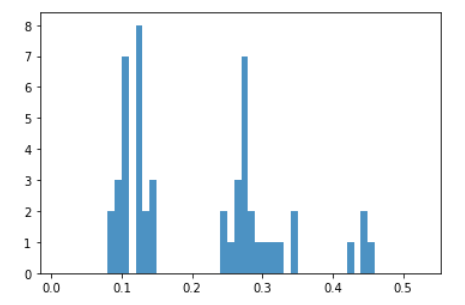
\includegraphics[scale=0.6]{graf.png}
\caption{Histogram 50 rezultatov silhuet.}
\label{slika1}
\end{center}
\end{figure}

Žal so ostali podatki o razvrščanju izgubljeni, jaz pa sem za to nalogo porabil že preveč dni.
Skupine se mi razvrstile podobno kot pri Hierarhičnem razvrščanju in so imele smisel.

\newpage


\section{Napovedovanje jezika.}
Za napovedovedovanje jezikov sem dodatno pridobil še po 2 edili za vsak jezik. Skupno 3 besedila so tvorila trojke pri vsakem jeziku.
Ko sem testiral odlomke besedil iz različnih jezikov, sem primerjal le-te z vsako trojko in izračunal povprečje ujemanja pri vseh treh.
Z nomalizacijo med dobljenimi vrednostmi za vseh 5 jezikov sem le-te pretvoril v procente verjetnosti ujemanja za posamezni jezik.
\\Jeziki, s katerimi sem primerjal odlomke so češčina, angleščina, španščina, madžarščina in slovenščina.


Tudi tu sem imel zelo lepe rezultate pa sem jih nevem kako pokvaril, da nič več nima smisla. Za stavek "Danes je lep dan" sem dobil pr ntrerkah dolžine 6 75\% verjetnost in
25\%, da je niz v češčini.
Na koncu sem ugotovil da sem rabil ponovno obrnit vrednost kosinusne razdalje, da sem imel opravka s podobnostjo in ne z razdaljo:
\\

Za španski odlomek o nogometu sem dobil vrednosti:
\\Odstavek: cada bando tiene su lugar de marca, en este caso las porterías son ruedas de molino incrustadas en el centro de unos muros de piedra. Estas están situadas a la orilla del río, separadas por una distancia de tres
{'si': 0.06493148413725684, 'es': 0.7924870045520438, 'ma': 0.05647705538723061, 'cz': 0.029139790533865693, 'en': 0.056964665389603035}
\\

Za slovensko poved "Danes je lep dan" sem dobil vrednosti:
\\Odstavek: Danes je lep dan
\\
{'si': 0.627352218875449, 'es': 0.1301125589299184, 'ma': 0.022638238037705254, 'cz': 0.19390214087943217, 'en': 0.025994843277495246}
\\

Za madžarski odlomek o luni sem dobil vrednosti:
\\Odlomek: A felszíni nehézségi gyorsulás (és így a testek súlya) körülbelül hatoda a földinek, így a rajta járó űrhajósok a 80–90 kg-os űrruhában is könnyedén mozogtak, ugráltak. A Holdnak nincsen számottevő légköre
\\
{'si': 0.044840778184110544, 'es': 0.04724704510075924, 'ma': 0.7505988139379031, 'cz': 0.10619303881221806, 'en': 0.051120323965009026}
\\

Za angleški odstavek o lesu sem dobil vrednosti:
\\Odstavek: Wood is sometimes defined as only the secondary xylem in the stems of trees,[1] or it is defined more broadly to include the same type of tissue elsewhere such as in the roots of trees or shrubs.
\\{'si': 0.08511081823308327, 'es': 0.07286592665435758, 'ma': 0.02464219738694819, 'cz': 0.026450289405044302, 'en': 0.7909307683205666}
\\


Za češki odstavek o pivu sem dobil vrednosti:
\\Odstavek: V současnosti je pivo konzumováno prakticky na celém světě. K roku 2008 drží obyvatelé Česka přední pozici v průměrné spotřebě piva na osobu, která dosahuje v průměru 160 litrů na hlavu za rok.
\\
{'si': 0.3803708169795609, 'es': 0.01679186185562227, 'ma': 0.013924444140972696, 'cz': 0.5756639433899943, 'en': 0.013248933633849984}
\\

Vidimo lahko, da so predikcije kar dobre. Edinokrat ko so procenti med sabo manj razmaknjeni je, ko imamo opravka s slovenskim ali češkim odlomkom.
\\Namreč jezika sta si podobna.




\end{document}
